\chapter{Método e Planeamento}

\section{Metodologia de Desenvolvimento}

O desenvolvimento deste projeto segue uma abordagem iterativa e incremental, adaptada ao contexto académico e às necessidades específicas do AISIC LAB. Esta escolha fundamenta-se na necessidade de validação contínua com stakeholders e na natureza evolutiva dos requisitos de uma ferramenta especializada para anotação de \textit{chat disentanglement}.

\subsection{Princípios Metodológicos}

A metodologia adotada assenta em três princípios fundamentais:

\begin{itemize}
    \item \textbf{Desenvolvimento Iterativo}: Ciclos de desenvolvimento flexíveis, permitindo adaptação às necessidades emergentes e feedback regular
    \item \textbf{Validação Contínua}: Envolvimento regular dos stakeholders do AISIC LAB para validação de funcionalidades
    \item \textbf{Desenvolvimento Incremental}: Construção progressiva da ferramenta, começando pelas funcionalidades essenciais de disentanglement
\end{itemize}

\subsection{Organização do Trabalho}

O desenvolvimento está estruturado em fases de trabalho, com os seguintes elementos:

\begin{itemize}
    \item \textbf{Planeamento}: Definição de objetivos e prioridades para cada fase de desenvolvimento
    \item \textbf{Desenvolvimento}: Implementação das funcionalidades priorizadas
    \item \textbf{Revisão}: Avaliação do progresso e demonstração aos stakeholders
    \item \textbf{Adaptação}: Análise do processo e ajustes necessários às circunstâncias
\end{itemize}

\section{Planeamento e Cronograma}

O planeamento do projeto, representado na Figura~\ref{fig:gantt-chart}, está organizado em fases distintas que refletem a evolução da ferramenta desde o protótipo inicial até à solução final.

\subsection{Fases do Projeto}

\subsubsection{Fase Inicial (Outubro - Dezembro 2024)}
Esta fase focou-se na validação de conceitos e estabelecimento de fundações:
\begin{itemize}
    \item Desenvolvimento do protótipo
    \item Validação da interface de anotação
    \item Levantamento tecnológico
    \item Documentação inicial
\end{itemize}

\subsubsection{MVP - Módulo Disentanglement (Dezembro 2024 - Janeiro 2025)}
Consolidação do protótipo existente:
\begin{itemize}
    \item Refinamento da interface frontend
    \item Testes de usabilidade
    \item Implementação de feedback inicial
    \item Validação com utilizadores piloto
\end{itemize}

\subsubsection{Infraestrutura Base (Janeiro - Março 2025)}
Estabelecimento da arquitetura da ferramenta:
\begin{itemize}
    \item Setup do ambiente de desenvolvimento
    \item Migração do backend para Python
    \item Implementação da arquitetura cliente-servidor
    \item Sistema de autenticação
\end{itemize}

\subsubsection{Ferramenta Principal (Março - Maio 2025)}
Desenvolvimento das funcionalidades principais:
\begin{itemize}
    \item Funcionalidades de anotação especializadas
    \item Sistema de gestão de datasets
    \item API para comunicação frontend-backend
    \item Interface de administração
\end{itemize}

\subsubsection{Finalização (Maio - Junho 2025)}
Preparação para disponibilização:
\begin{itemize}
    \item Testes extensivos
    \item Validação com utilizadores
    \item Documentação técnica
    \item Preparação para deployment
\end{itemize}

\section{Análise Crítica ao Planeamento}

A presente secção visa analisar o progresso do projeto face ao planeamento inicial, identificando os principais marcos alcançados, os desafios encontrados e as adaptações realizadas durante o desenvolvimento.

\subsection{Progresso Realizado}
Desde a validação inicial do conceito através do protótipo, o desenvolvimento focou-se na construção da infraestrutura base e das funcionalidades principais de \textit{chat disentanglement}. Os principais avanços incluem:
\begin{itemize}
    \item Implementação do \textit{backend} utilizando a framework FastAPI em Python, estabelecendo uma API REST para comunicação com o \textit{frontend}.
    \item Configuração da persistência de dados com uma base de dados SQLite, gerida através do ORM SQLAlchemy.
    \item Desenvolvimento e integração do sistema de autenticação e gestão de utilizadores com papéis (administrador/anotador).
    \item Refinamento e desenvolvimento contínuo do \textit{frontend} em React, implementando as interfaces necessárias para a gestão de projetos e a anotação de \textit{disentanglement}.
    \item Implementação da funcionalidade de importação de dados a partir de ficheiros CSV.
    \item Desenvolvimento do algoritmo de cálculo automático de métricas de concordância inter-anotador.
\end{itemize}
Este progresso permitiu obter uma versão funcional da ferramenta centrada na sua tarefa principal, conforme pode ser visualizado no cronograma atualizado (Figura~\ref{fig:gantt-chart}).

\subsection{Desafios Encontrados e Adaptações ao Plano}
Durante o desenvolvimento, alguns desafios e constrangimentos levaram a ajustes no plano e na abordagem inicial:

\begin{itemize}
    \item \textbf{Priorização vs. Generalidade:} A visão inicial de uma plataforma altamente modular, capaz de suportar diversos tipos de anotação de forma extensível, revelou-se demasiado ambiciosa para o âmbito temporal e os recursos disponíveis no TFC. Para garantir a entrega de uma solução funcional e útil para o caso de uso principal do AISIC Lab, foi tomada a decisão consciente de **priorizar o desenvolvimento especializado para \textit{chat disentanglement}**. Isto implicou que a implementação do \textit{backend} e do modelo de dados fosse mais específica para esta tarefa, permitindo uma maior qualidade e adequação da solução final.
    \item \textbf{Foco em Formatos Essenciais:} Pelas mesmas razões de priorização e alinhamento com as necessidades imediatas do caso de uso, o suporte foi centrado nos formatos mais relevantes: importação através de CSV e exportação em JSON. O suporte a outros formatos de importação de dados permanece como um objetivo para evolução futura.
    \item \textbf{Complexidade Técnica:} A integração entre o frontend e o backend, a gestão do estado da aplicação e a implementação correta das interações de anotação apresentaram desafios técnicos que exigiram tempo e esforço de desenvolvimento significativo.
    \item \textbf{Balanceamento de Funcionalidades:} Foi necessário balancear o desenvolvimento de novas funcionalidades com a necessidade de refinar e estabilizar as funcionalidades existentes. Este processo incluiu também a resposta a feedback e requisitos que emergiram durante o desenvolvimento.
    \item \textbf{Adaptação do Processo:} O processo de desenvolvimento teve de ser adaptado às circunstâncias académicas, com períodos de maior e menor intensidade de trabalho, ajustando-se às necessidades de outras disciplinas e compromissos académicos.
\end{itemize}
Estas adaptações, embora desviando da visão mais abrangente inicial, foram consideradas necessárias para garantir a viabilidade da entrega de um produto funcional e relevante dentro do contexto do TFC. A especialização para \textit{chat disentanglement} permitiu uma maior qualidade e adequação da solução às necessidades específicas identificadas.

\subsection{Implicações no Planeamento Futuro}
As decisões de priorização refletem-se no estado atual da ferramenta e no planeamento subsequente. O foco continuará a ser a consolidação e teste das funcionalidades de \textit{disentanglement}. A introdução de maior generalidade no backend e o suporte a outros formatos de dados são agora considerados trabalhos futuros, a serem abordados após a validação e estabilização da funcionalidade principal. A documentação técnica e os testes de usabilidade (Capítulo 5) ganharam maior ênfase para garantir a qualidade da entrega atual.

O desenvolvimento demonstrou que uma abordagem pragmática, focada na entrega de valor específico para o domínio de \textit{chat disentanglement}, é mais eficaz que uma tentativa de criar uma solução genérica sem validação adequada das necessidades específicas.

\begin{landscape}
    \begin{figure}[p]
        \centering
        \makebox[\textwidth][c]{%
            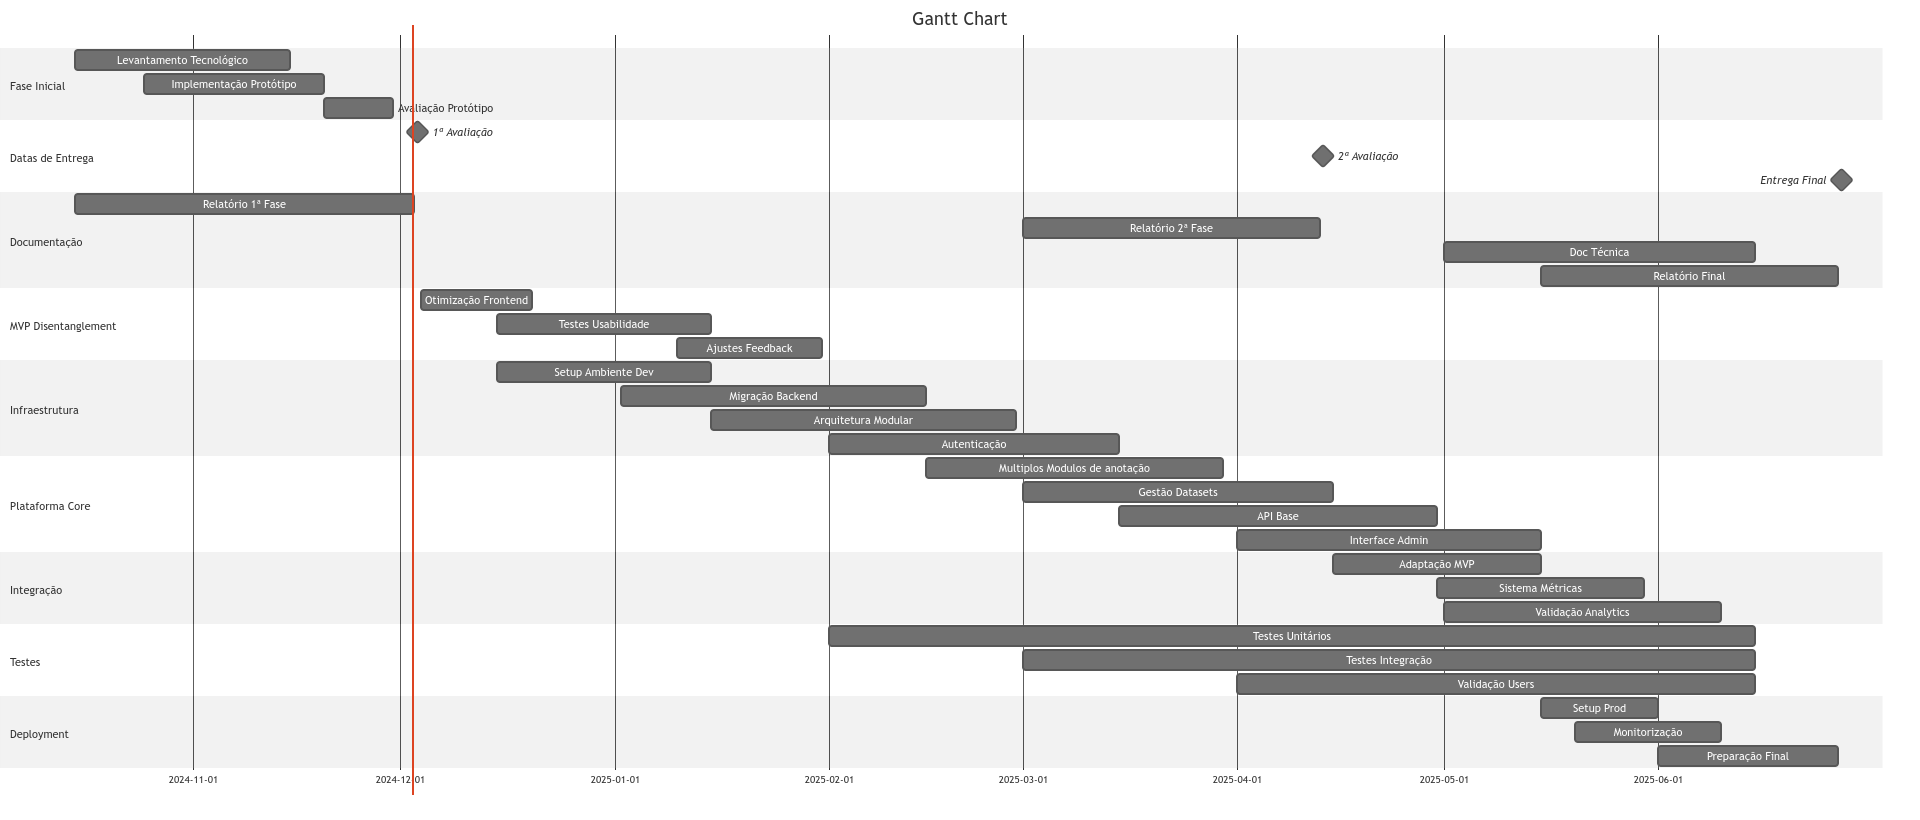
\includegraphics[width=0.98666\paperheight, angle=0, keepaspectratio]{images/Gant.drawio.png}
        }
        \caption{Cronograma detalhado do projeto (Gantt Chart) - Estado Atualizado}
        \label{fig:gantt-chart}
    \end{figure}
\end{landscape}
